\documentclass[MScCS]{uccthesis}

\title{Rational Bloom Filters}
\author{Ross Heaney}
\supervisor{Dr Marc Van Dongen}
\secondreader{Dr Who}
\date{\today}

\newcommand*{\COMMAND}[1]{\texttt{\textbackslash #1}}
\newcommand*{\COMMANDWITHARGUMENT}[2]{\texttt{\textbackslash #1}\{#2\}}

\addbibresource{mybib.bib}% should be in preamble

\abstract{%
Bloom Filters are a type of space-efficient probabilistic data structure that can be used to test whether an element is a member of a set. That is when the Bloom Filter is queried 'does this element exist in the set?' and the Bloom Filter returns 'yes' when in fact the element does not exist in the set. We accept these false positives as by agreeing to occasionally get a false positive, we gain an enormous space advantage versus had we refused to accept a false positive.  Using mathematics we can know in advance our false positive rate and tune the bloom filter accordingly. Namely, by setting the size of our bit array to $\frac{K}{S}\ln(2)$ we can reduce the false positive rate of the bloom filter to $2^{-K}$, which is optimal. Given a maximum, allowed false positive rate, r, finding the optimal (minimal) value for k is easy. By assumption k is integral, which makes it difficult to tune a Bloom filter when the desired false positive rate is almost of the form $2^{-k}$. For example, a small change in r may result in a significant increase in the size of the filter, especially when k is small. This thesis is about relaxing this integrality assumption and comparing to the state of the art.
}

%\dedication{%
%   Your dedication here.
%}

%\acknowledgement{%
%   Your acknowledgement here.
%}

\renewcommand\addToFrontMatter[0]{%
}

\begin{document}
\chapter{Introduction}

Bloom Filters are a type of space-efficient probabilistic data structure that can be used to test whether an element is a member of a set. They have exploded in popularity as their usefulness is proportional to the size of the membership set. That is, the larger the size of the dataset we wish to query, the more useful Bloom Filters are. With ever-increasing amounts of data being produced and pipelined year after year, the more Bloom Filters have become almost necessary. In this first chapter I will discuss my thesis mission and the literature review plan. I then follow on with the background and related work in chapter 2. Specifically I discuss the origins of the Bloom Filter via the original paper by Bloom\cite{bloom1970space} and discuss important mathematical results by Kirsch and Mitzenmacher as well as a small but important detail from the book by Mitzenmacher and Upfal\cite{kirsch2006less}\cite{mitzenmacher2017probability}.

\section{Motivations}
As mentioned in the Introduction, bloom filters are a type space efficient probabilistic data structure. First conceived in the 1970s, Bloom Filters have seen widespread use ever since. Today they are used in a variety of applications, including network security, distributed systems, and databases. As data gets larger and larger it becomes more and more difficult to store and process it. Bloom Filters are a way to store and process data in a space efficient manner. This is done by using the so called 'Allowable Error Hashing' technique proposed in the landmark paper, by Burton Howard Bloom, in 1970\cite{bloom1970space}. This technique allows for a trade-off between the space efficiency and the accuracy of the data structure. More importantly, we can tune and optimize the Bloom Filter in relation to the accuracy and space efficiency of the data structure. Specifically this project and thesis titled 'Rational Bloom Filters' will focus on looking at new ways to tune and optimize the Bloom Filter with a specific focus on relaxing the integrality assumption of the number of hash functions required for the Bloom Filter to function properly.

\section{Thesis Mission}
Bloom Filters are based on hashing. Specifically hashing where we accept there will be some hash collisions that will give rise to so called 'false positives'. That is when the Bloom Filter is queried 'does this element exist in the set?' and the Bloom Filter returns 'yes' when in fact the element does not exist in the set. We accept these false positives as by agreeing to occasionally get a false positive, we gain an enormous space advantage versus had we refused to accept a false positive.  Using mathematics we can know in advance our false positive rate and tune the bloom filter accordingly. Namely, by setting the size of our bit array to $\frac{K}{S}\ln(2)$ we can reduce the false positive rate of the bloom filter to $2^{-K}$, which is optimal. Given a maximum, allowed false positive rate, r, finding the optimal (minimal) value for k is easy. By assumption k is integral, which makes it difficult to tune a Bloom filter when the desired false positive rate is almost of the form $2^{-k}$. For example, a small change in r may result in a significant increase in the size of the filter, especially when k is small. This thesis is about relaxing this integrality assumption and comparing to the state of the art.

\chapter{Background and Literature Review}
In this chapter I will discuss the background and related work in the area of bloom filters. Specifically I will discuss the concept of a bloom filter before discussing the original paper by Bloom and the recent work done on bloom filters as it relates to this thesis. Throughout, I will be discussing important mathematical results that are relevant to the thesis.
\section{Concept of a Bloom Filter}
The concept of a bloom filter is summarized nicely in this diagram \ref{fig:bloomfilter}. The core idea behind bloom filters is the concept of hashing. Hashing is simply the transformation of an input value to an output value. In a bloom filter, sometimes a different input will transform to the same output. This is called a hash collision. In certain use cases such as cryptography, hash collisons can be very dangerous, but in the case of Bloom Filters, we accept hash collisions. So, naturally the question is why do we allow hash collisons in Bloom Filters? The answer to that question is space efficiency. By allowing hash collisions we can reduce the space required to store the data structure. This will be discussed in more detail in the next section. For now, it is important to note that the core idea behind a bloom filter is the concept of hashing and allowing hash collisions. The core use case of a Bloom Filter is testing set membership. This is where we can query whether 'x' is present in the Bloom Filter or not. The Bloom Filter will respond either "possibly in the set" or "definitely not in the set". The Bloom Filter will never return a \textit{false negative} but \textit{false positives} are possible.

\begin{figure}[h]
    \centering
    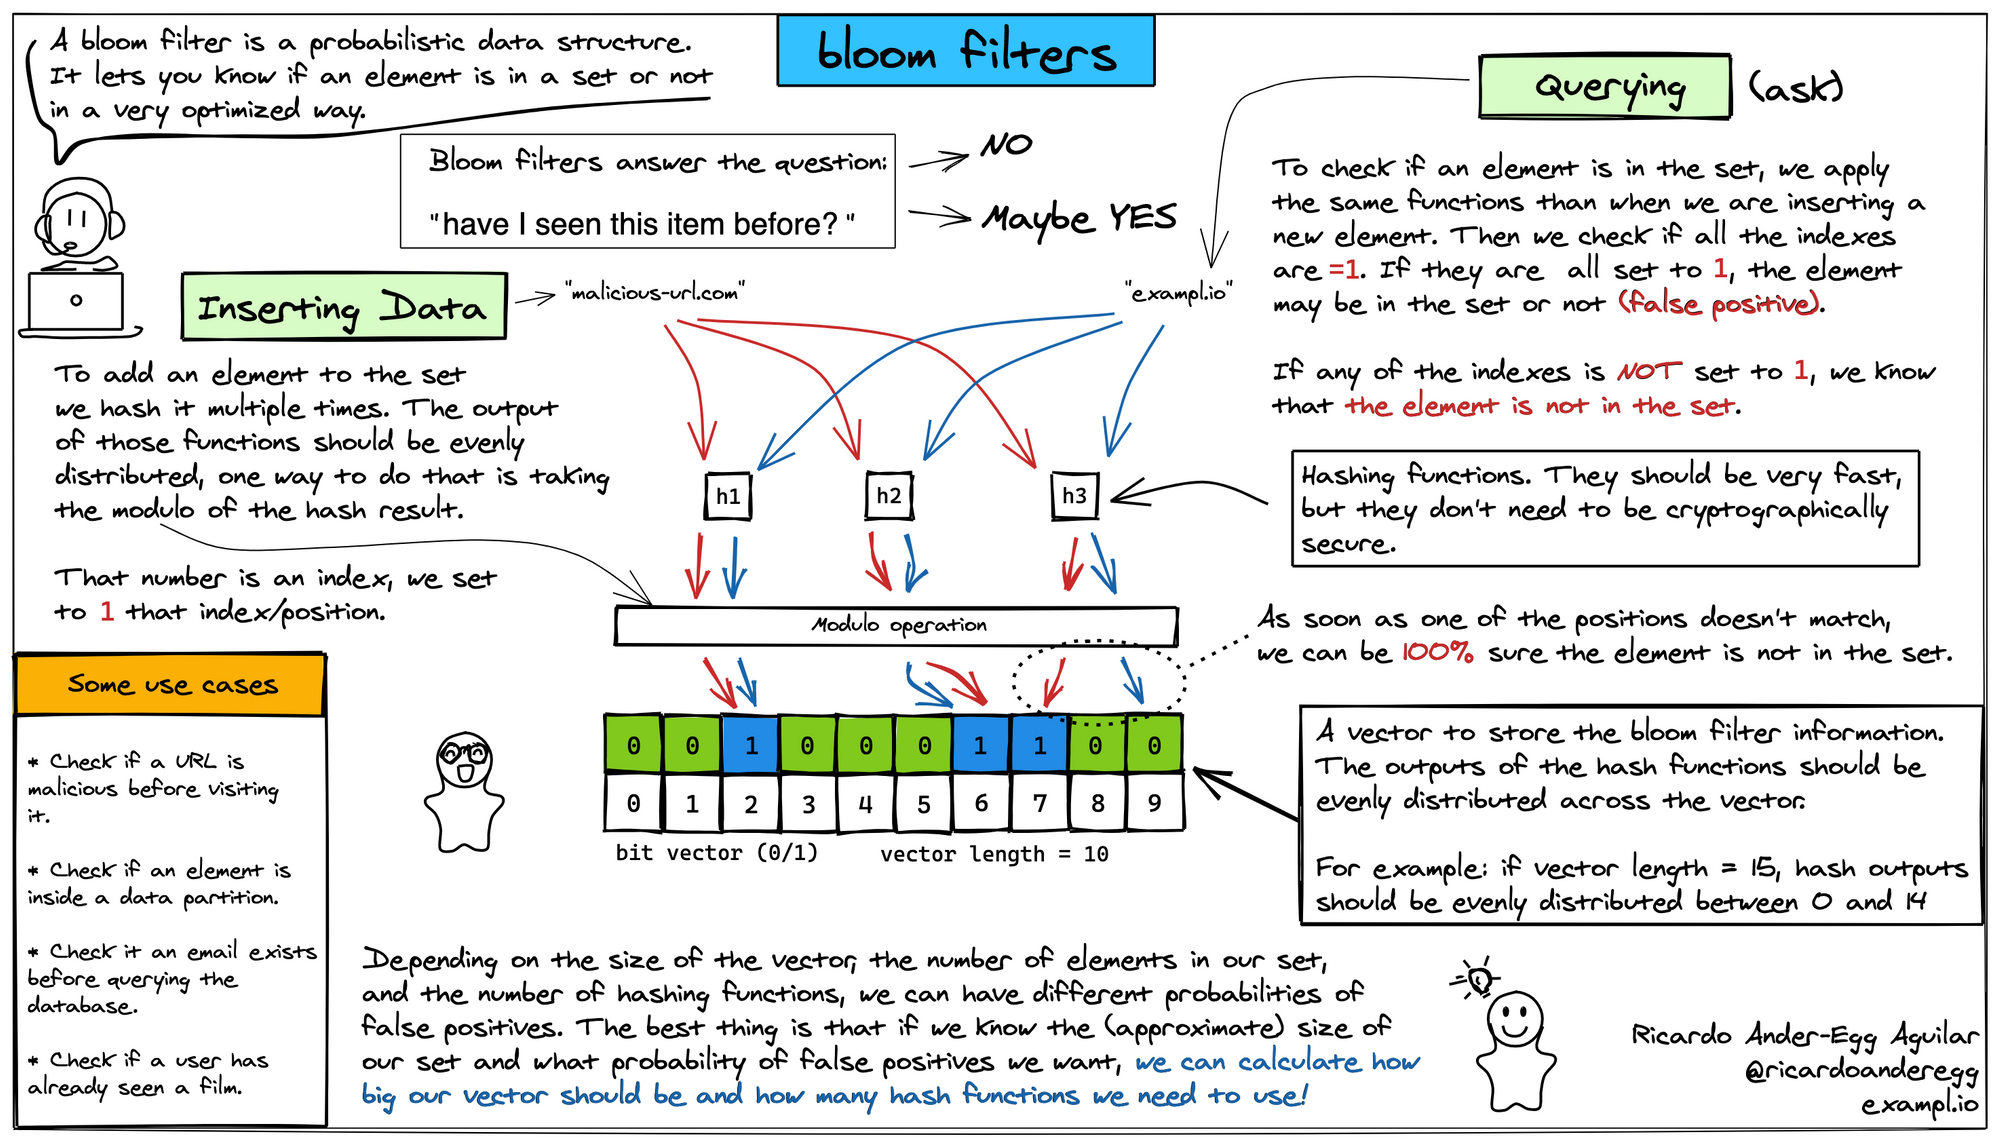
\includegraphics[width=\linewidth]{figures/bloom-filters-poster.png}
    \caption{Bloom Filter Summary}
    \label{fig:bloomfilter}
\end{figure}

\begin{figure}[h]
    \centering
    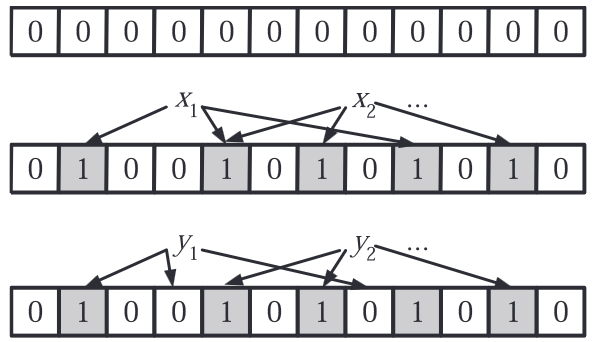
\includegraphics[width=\linewidth]{figures/bloom_filter_example.png}
    \caption{An example of a bloom filter taken from \cite{broder2004network}.The filter begins as an array of all 0s. Each item in the set xi is hashed k times, with each hash yielding a bit location; these bits are set to 1. To check if an element y is in the set, hash it k times and check the corresponding bits. The element y1 cannot be in the set, since a0 is found at one of the bits. The element y2 is either in the set or the filter has yielded a false positive.}
    \label{fig:bloomfilterExample}
\end{figure}



\section{Original Paper by Burton Howard Bloom}
The paper was the first paper to introduce the idea of \textit{Allowable Error Hashing}, which is the basis of Bloom Filters. The essence of Bloom Filters is that set membership, is this item in this set?, can be answered in one of two ways. The first way is to return \underline{yes this item is in the set} and the other way is to say \underline{no this item is not in the set}. Bloom Filters \textbf{guarantee} that false negatives are not possible, while occasionally a false positive is possible. In other words when a Bloom Filter is queried whether an item is in the set or not, it will return "possibly in the set" or "definitely not in the set". The underlying mechanism for the construction of a Bloom Filter is a number of hash functions that map elements of a set to indices on an array. This can be seen in Figure \ref{fig:bloomfilter}. The paper introduced the key concept of an \textit{Allowable Error Rate}. By accepting that we will get a false positive occasionally, we can achieve remarkable space efficiency. The paper's proposed idea is analysed quite nicely via a mathematical comparison between the conventional error-free hashing, state of the art in the 1970s, and the authors proposed \textit{Allowable Error Hashing}. It should be noted that some errors have been found in the original paper and updates published\cite{bose2008false}. The errors found are mostly to do with edge cases and do not necessarily diminish the original paper's contribution. The paper discusses an example of a hyphenation algorithm. Suppose we have a dictionary of 500,000 words of which 90\% follow simple hyphenation rules but the remaining 10\% require expensive disk access to retrieve very specific hyphenation rules that are stored on the disk. By applying the authors \textit{Allowable Error Hashing} technique, disk access is greatly reduced. A hash area only 15\% of the total size needed by an error-free hash cuts down on 85\% of the disk access required. The main idea is not that error-free hashing is bad but rather there is a proposed alternative called \textit{Allowable Error Hashing} that is better suited to certain applications.

\section{Less Hashing, Same Performance}
he paper by  Kirsch and Mitzenmacher \cite{kirsch2006less} is a very nice paper that discusses the number of necessary hash functions to implement a Bloom Filter without any loss in asymptotic false positive probability. Specifically the paper proves a mathematical result that only two hash functions are necessary to implement the Bloom Filter. This paper is \textbf{not} saying that only two hash functions are all that is required for all Bloom Filters, rather that in certain cases only two hash functions are required. This is a vitally important result as it means we can limit our computation overhead and maintain the same performance. Bloom filters are randomized data structures as they rely on pseudorandom hash functions. By reducing the number of hash functions needed then this cuts down on much of the non-trivial computation required to create a Bloom Filter. The important result that was proved in this paper is the following mathematical statement: $(1-e^\frac{-kn}{m})^k$, where m is array size in bits, n is the number of elements in the m size array and k is the number of hash functions. This formula gives us the approximate probability of false positives but Mitzenmacher did it without the assumption of independence, an important distinction from previous mathematical analysis done in other papers. Also related, The book by Mitzenmacher and Upfal \cite{mitzenmacher2017probability} is a very nice book on probability and computing that discusses Bloom Filters in a dedicated subchapter. The important takeaway from the chapter among many other things is that the if you have an m-bit Bloom filter with n elements inserted, then the optimal number k of hash functions to use is $k = \frac{m}{n}\ln 2$.

\section{Network Applications of Bloom Filters}
This paper\cite{broder2004network} discusses some very interesting applications for Bloom Filters, and it's an important paper to get a better understanding of Bloom Filters and their uses. Specifically it discusses four instances of network related applications for Bloom Filters
\begin{itemize}
    \item Collaborating in overlay and peer-to-peer networks
    \item Resource routing
    \item Packet routing
    \item Network measurement
\end{itemize}
Specifically what I learned from the paper is that Bloom Filters can play an important role in the optimization of networks. But more importantly the paper stresses there is a lot of room for innovation and improvement regarding Bloom Filters in the area of networking and the above list of network related applications involving Bloom Filters is not exhaustive, rather it is a starting point.


\section{Probability and Computing by Mitzenmacher and Upfal}
The chapter dedicated to Bloom filters in the fantastic book Probability and Computing by Mitzenmacher and Upfal \cite{mitzenmacher2017probability} is a very nice chapter that discusses Bloom Filters in a dedicated subchapter. The important takeaway from the chapter among many other things is that the if you have an m-bit Bloom filter with n elements inserted, then the optimal number k of hash functions to use is $k = \frac{m}{n}\ln 2$.

\section{Partitioned learned bloom filter}
The paper by Vaidya et al. \cite{vaidya2020partitioned} is a very interesting paper that discusses the use of Bloom Filters in the context of

\cite{vaidya2020partitioned}
\section{Adaptive Learned Bloom Filters}
The paper by Dai et al. \cite{dai2019adaptive} is a very interesting paper that discusses the use of Bloom Filters in the context of
\cite{dai2019adaptive}

\section{Optimizing bloom filter: Challenges, solutions, and comparisons}
The paper by Dai et al. \cite{dai2019optimizing} is a very interesting paper that discusses the use of Bloom Filters in the context of
\cite{dai2019optimizing}

%
%
\backmatter
%
%
\printbibliography
\end{document}
